\section{Superposition}
\label{sec:superposition}

\begin{sessioncard}
\textbf{Session 4.} \emph{Goal:} understand why single neurons are usually hard to interpret, and learn the
hypothesis that explains this: a network stores more features than it has dimensions.
\emph{Experiments:} what single neurons of GPT-2 small respond to (\cref{exp:neurons}), how close to orthogonal
random directions are (\cref{exp:random}), and a small model, trained from scratch, that starts to use
superposition when its features become sparse (\cref{exp:pentagon,exp:toytwo}).
\emph{Prerequisites:} session 3. The proofs use one inequality from probability theory.
\end{sessioncard}

\subsection{Neurons respond to many things}

If features are directions, the most convenient directions for us would be the coordinate axes of some layer.
In the stream, the coordinates play no special role. The neurons of an MLP, however, do play a special role,
because the nonlinearity acts on each neuron separately. So we might hope that each neuron represents one feature.
The next experiment tests this hope.

\begin{experiment}[Three neurons of GPT-2 small]\label{exp:neurons} \script{exp\_neurons.py}
We record the activations of the $3072$ neurons of the MLP of layer 6 on $38{,}100$ tokens of text. We say that
a neuron \emph{fires} on a token if it is strongly active on this token. For each neuron, we look at the ten tokens
on which it fires most strongly. \Cref{tab:neurons} shows three neurons. Neuron 35 is easy to interpret: it fires
on the plural endings of abbreviations and technical terms. Neuron 0 fires on parts of capitalised names in program
code, on the names of weekdays, and on the second half of compound words such as \tok{four-year}. Neuron 26 fires on
a collection of words that have no visible connection. With the option \texttt{--explore}, the script prints the
same list for the first forty neurons of the layer, so that the seminar can judge how common each of the three
kinds is. In our judgement, neurons like neuron 35 are the exception.
\end{experiment}

\begin{table}[t]
\centering\small
\begin{tabular}{@{}l>{\raggedright\arraybackslash}p{0.82\textwidth}@{}}
\toprule
Neuron & Tokens with the strongest activation (in brackets), with the text before them \\
\midrule
6.35 & \tok{RPD[s]}, \tok{(MS[Us]}, \tok{Aux[ins]}, \tok{WIM[Ps]}, \tok{(FPTC[s]}, \tok{olig[omers]},
\tok{(EM[Ms]}, \tok{N[Vs]}, \tok{apparat[uses]} \\ \addlinespace
6.0 & \tok{NS\_ASS[UME]}, \tok{thirty-[man]}, \tok{on[ Saturday]}, \tok{COMM[ITT]}, \tok{extended.[ By]},
\tok{on[ Tuesday]}, \tok{four-[year]}, \tok{38-[minute]}, \tok{BOO[ST]} \\ \addlinespace
6.26 & \tok{next[ door]}, \tok{located[ near]}, \tok{was the[ daughter]}, \tok{were[ local]},
\tok{our[ partner]}, \tok{Plaintiff[-]}, \tok{come[ face]}, \tok{foot[-]} \\
\bottomrule
\end{tabular}
\caption{Three neurons of the MLP of layer 6 of GPT-2 small (\cref{exp:neurons}).}
\label{tab:neurons}
\end{table}

A neuron that responds to several unrelated things is called \emph{polysemantic}. Polysemantic neurons were the
main obstacle for early research in interpretability. The \emph{superposition hypothesis} \citep{elhage2022toy}
explains them: the network represents many more features than it has neurons, so not every feature can have a
neuron of its own.

\subsection{More directions than dimensions}

How can a space of dimension $d$ hold more than $d$ features? If the feature directions of \cref{def:lrh} had to
be orthogonal, this would be impossible, because $\R^d$ contains at most $d$ orthogonal unit vectors. But the
directions only need to be \emph{almost} orthogonal, and the following proposition shows that there are very many
almost orthogonal directions.

\begin{proposition}[Many almost orthogonal directions]\label{prop:jl}
Let $0<\varepsilon<1$ and let $N\ge 2$ be an integer with $N\le\exp(\varepsilon^2d/4)$. Then there are unit
vectors $v_1,\dots,v_N\in\R^d$ with $|v_i^\top v_j|\le\varepsilon$ for all $i\ne j$.
\end{proposition}
\begin{proof}
We choose the vectors at random and show that they have the property with positive probability. Let all $dN$
coordinates of $v_1,\dots,v_N$ be independent, each equal to $+1/\sqrt d$ or $-1/\sqrt d$ with probability $1/2$.
Every $v_j$ then has norm one.

\textbf{One pair.} Fix $i\ne j$. The number $d\,v_i^\top v_j$ is a sum of $d$ terms, one for each coordinate, and
each term is the product of two independent uniform random signs. Such a product is again a uniform random
sign, and the $d$ terms are independent because the coordinates are. Hoeffding's inequality
\citep[Theorem 2]{hoeffding1963probability} states that a sum of $d$ independent random variables with values in
$[-1,1]$ and mean zero is at least $\varepsilon d$ with probability at most $\exp(-(\varepsilon d)^2/(2d))$. We
use it for the sum $d\,v_i^\top v_j$ and for its negative:
\begin{align}
\Pr\big(|v_i^\top v_j|>\varepsilon\big)
&\le \Pr\big(d\,v_i^\top v_j\ge\varepsilon d\big)+\Pr\big(-d\,v_i^\top v_j\ge\varepsilon d\big) && \by{union of two events}\notag\\
&\le 2\exp\!\big(-(\varepsilon d)^2/(2d)\big) && \by{Hoeffding, twice}\notag\\
&= 2\exp\!\big(-\varepsilon^2d/2\big). && \by{simplifying the exponent} \label{eq:onepair}
\end{align}

\textbf{All pairs.} There are $N(N-1)/2$ pairs $i<j$. Hence
\begin{align*}
\Pr\big(\text{some pair has }|v_i^\top v_j|>\varepsilon\big)
&\le \frac{N(N-1)}{2}\cdot 2\exp\!\big(-\varepsilon^2d/2\big) && \by{union bound and \eqref{eq:onepair}}\\
&< N^2\exp\!\big(-\varepsilon^2d/2\big) && \by{since $N(N-1)<N^2$}\\
&\le \exp\!\big(\varepsilon^2d/2\big)\exp\!\big(-\varepsilon^2d/2\big) && \by{since $N\le\exp(\varepsilon^2d/4)$}\\
&= 1. && \by{the two exponents cancel}
\end{align*}
The probability that some pair violates the bound is strictly smaller than one. So there is an outcome in
which no pair violates it, and this outcome is the required family of vectors.
\end{proof}

For $d=768$ and $\varepsilon=0.3$, the proposition gives more than $3\times10^7$ directions, compared with only
$768$ exactly orthogonal directions. The constants in the proposition are far from optimal. What matters is that
the number of directions grows exponentially with $d$.

\begin{experiment}[Random directions are almost orthogonal]\label{exp:random} \script{exp\_superposition.py}
We can observe the idea of the proof directly. We draw $2000$ random unit vectors in $d=768$ dimensions and
compute the inner products of all pairs. This gives about two million numbers (\cref{fig:random}). Their standard
deviation is $0.036$, which equals $1/\sqrt{768}$. The largest absolute value among all pairs is $0.17$, and only
$0.5\%$ of the pairs have an absolute value above $0.1$. So random directions in a high-dimensional space are almost
orthogonal, without any optimisation.
\end{experiment}

\begin{figure}[t]
\centering
\begin{minipage}[c]{0.55\textwidth}
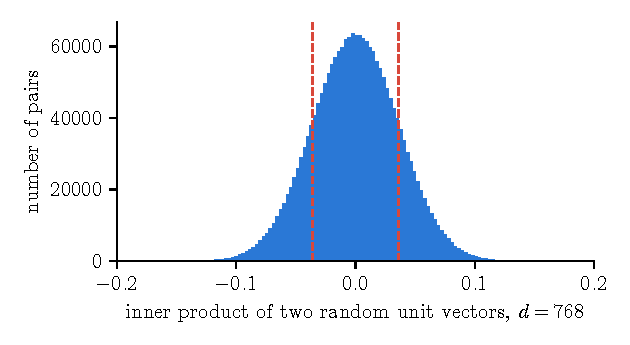
\includegraphics[width=\textwidth]{figures/fig_random_cosines.pdf}
\end{minipage}\hfill
\begin{minipage}[c]{0.4\textwidth}
\caption{Inner products of all pairs among $2000$ random unit vectors in $768$ dimensions (\cref{exp:random}).
The dashed lines mark $\pm1/\sqrt{768}$.}
\label{fig:random}
\end{minipage}
\end{figure}

However, almost orthogonal directions are not exactly orthogonal, and this has a cost, called
\emph{interference}. If we read feature $j$ from $x$ by projecting $x$ onto $v_j$, the other active features add
small errors to the result. The following lemma bounds these errors.

\begin{lemma}[Interference is controlled by sparsity]\label{lem:interference}
Let $v_1,\dots,v_N$ be unit vectors with $|v_i^\top v_j|\le\varepsilon$ for $i\ne j$. Let $x=\sum_{i=1}^{N}f_iv_i$,
where at most $k$ of the numbers $f_1,\dots,f_N$ are nonzero and all of them lie in $[0,1]$. Then
$|v_j^\top x-f_j|\le k\varepsilon$ for every $j$.
\end{lemma}
\begin{proof}
We expand $v_j^\top x$ and bound the terms with $i\ne j$.
\begin{align*}
|v_j^\top x-f_j| &= \Big|\sum_{i=1}^{N}f_i\,v_j^\top v_i-f_j\Big| && \by{definition of $x$}\\
&= \Big|\sum_{i\ne j}f_i\,v_j^\top v_i\Big| && \by{since $v_j^\top v_j=1$}\\
&\le \sum_{i\ne j}f_i\,|v_j^\top v_i| && \by{triangle inequality, $f_i\ge0$}\\
&\le k\varepsilon. && \by{at most $k$ nonzero terms, each at most $\varepsilon$}\qedhere
\end{align*}
\end{proof}

The lemma shows what superposition needs: \emph{sparsity}. Storing many features in few dimensions causes little
harm, as long as only a few features are active at the same time. Most features of language are of this kind. For
example, the feature ``this text is about the Golden Gate Bridge'' is absent from almost all texts. A nonlinearity
can then remove the remaining interference. If feature $j$ is absent, the lemma gives $v_j^\top x\le k\varepsilon$,
and therefore $\relu(v_j^\top x-k\varepsilon)=0$. So a $\relu$ with a threshold reports an absent feature as
exactly absent.

\subsection{A toy model, trained from scratch}
\label{sec:toy}

We now know that superposition is possible. Does gradient descent actually find such arrangements of directions?
\citet{elhage2022toy} study this question in a very small network. There are $N$ features with activations
$f=(f_1,\dots,f_N)$. The features are independent. Each $f_j$ is zero with probability $1-\delta$, and it is
uniformly distributed on $[0,1]$ with probability $\delta$. So a small $\delta$ means that the features are sparse.
The model compresses $f$ into $d<N$ dimensions and then tries to recover $f$:
\begin{equation}\label{eq:toy}
x \;=\; Wf\in\R^d,\qquad \hat f \;=\; \relu\big(W^\top x+b_{\mathrm{toy}}\big)\in\R^N,\qquad
\text{loss} \;=\; \E\sum_{j=1}^{N}I_j\,\big(f_j-\hat f_j\big)^2 ,
\end{equation}
with a weight matrix $W\in\R^{d\times N}$, a bias vector $b_{\mathrm{toy}}\in\R^N$ and fixed positive weights
$I_j$ that state how important each feature is. Column $j$ of $W$ is the direction that the model uses for feature
$j$. If column $j$ is zero, feature $j$ is not represented at all.

\begin{experiment}[Five features in two dimensions]\label{exp:pentagon} \script{exp\_superposition.py}
We train the model \eqref{eq:toy} with $N=5$, $d=2$ and importances $I_j=0.7^{\,j-1}$, for three values of
$\delta$, and we draw the five columns of $W$ as arrows in the plane (\cref{fig:toygeometry}). When all features are
always active, the model represents the two most important features in orthogonal directions, and it gives the
other three features no direction at all. When the features are active $20\%$ of the time, the model represents
four features, as two pairs of opposite directions. When they are active $5\%$ of the time, it represents all five
features, arranged as a pentagon. So the same network, trained in the same way, uses superposition when its
features are sparse and does not use it when they are dense.
\end{experiment}

\begin{figure}[t]
\centering
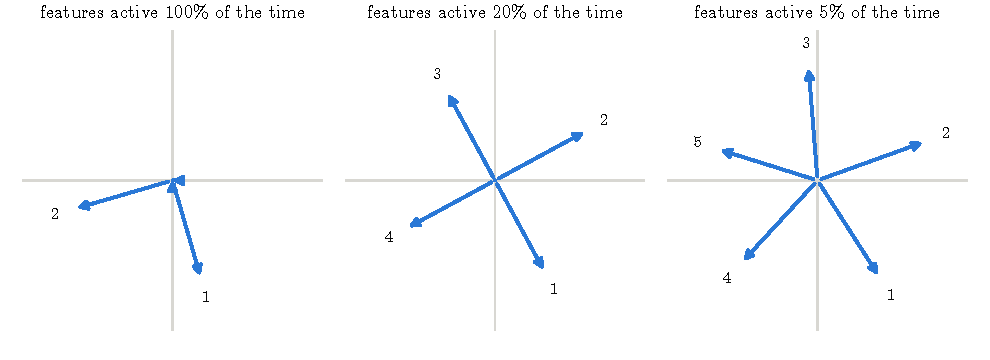
\includegraphics[width=0.92\textwidth]{figures/fig_toy_geometry.pdf}
\caption{The directions that a trained toy model assigns to five features in two dimensions, for three levels
of sparsity (\cref{exp:pentagon}). The numbers order the features by importance.}
\label{fig:toygeometry}
\end{figure}

The smallest case can be solved by hand, and the calculation explains why the model changes its behaviour. Let
$N=2$, $d=1$ and $I_1=I_2=1$. The model has a single number $x$ in which to store two features. We compare two ways
of doing this.
\begin{itemize}
\item \textbf{Dedicated solution.} $W=(1,\ 0)$ and $b_{\mathrm{toy}}=(0,\ \delta/2)$. The model stores feature $1$
and ignores feature $2$, for which it always outputs the constant $\delta/2$.
\item \textbf{Antipodal solution.} $W=(1,\ -1)$ and $b_{\mathrm{toy}}=(0,\ 0)$. The model stores the difference
$x=f_1-f_2$. For example, the input $f=(0.6,\ 0.2)$ is stored as $x=0.4$ and read back as $\hat f=(0.4,\ 0)$.
\end{itemize}

\begin{proposition}[Superposition wins when features are sparse]\label{prop:toy}
In the model \eqref{eq:toy} with $N=2$, $d=1$, $I_1=I_2=1$ and $0<\delta\le1$, the dedicated solution has loss
$\delta/3-\delta^2/4$ and the antipodal solution has loss $\delta^2/3$. The antipodal solution has the smaller
loss if and only if $\delta<4/7$.
\end{proposition}
\begin{proof}
We use that a variable which is uniform on $[0,1]$ has mean $1/2$ and second moment $1/3$. Hence
$\E f_2=\delta/2$ and $\E f_2^2=\delta/3$.

\textbf{Dedicated solution.} Here $x=f_1$, so $\hat f_1=\relu(f_1)=f_1$ and $\hat f_2=\relu(\delta/2)=\delta/2$.
\begin{align*}
\text{loss} &= \E\big(f_1-f_1\big)^2+\E\big(f_2-\delta/2\big)^2 && \by{inserting $\hat f_1$ and $\hat f_2$}\\
&= \E f_2^2-\delta\,\E f_2+\delta^2/4 && \by{expanding the square}\\
&= \delta/3-\delta^2/2+\delta^2/4 && \by{since $\E f_2=\delta/2$, $\E f_2^2=\delta/3$}\\
&= \delta/3-\delta^2/4. && \by{collecting the terms with $\delta^2$}
\end{align*}

\textbf{Antipodal solution.} Here $x=f_1-f_2$, so $\hat f_1=\relu(f_1-f_2)$ and $\hat f_2=\relu(f_2-f_1)$. If
$f_2=0$, then $\hat f_1=f_1$ and $\hat f_2=\relu(-f_1)=0=f_2$, and the error is zero. The same holds if $f_1=0$.
The only inputs with an error are those with both features active, which has probability $\delta^2$. Let both
be active and let $f_1\ge f_2$. Then $\hat f_1=f_1-f_2$ and $\hat f_2=0$, so both errors equal $f_2$ and the
squared error is $2f_2^2=2\min(f_1,f_2)^2$. For $f_2\ge f_1$ we obtain the same expression by symmetry. Given that
both features are active, $f_1$ and $f_2$ are independent and uniform on $[0,1]$, so
$\Pr(\min(f_1,f_2)>u)=(1-u)^2$ and the minimum has density $2(1-u)$ on $[0,1]$.
\begin{align*}
\text{loss} &= \delta^2\cdot 2\int_0^1u^2\cdot 2(1-u)\,du && \by{error only if both active}\\
&= \delta^2\cdot 4\Big(\frac13-\frac14\Big) && \by{since $\textstyle\int_0^1u^2du=\frac13$, $\int_0^1u^3du=\frac14$}\\
&= \frac{\delta^2}{3}. && \by{since $\textstyle\frac13-\frac14=\frac1{12}$}
\end{align*}

\textbf{Comparison.} Dividing by $\delta>0$, we get
$\delta^2/3<\delta/3-\delta^2/4$ exactly if $\delta/3+\delta/4<1/3$, which means $\delta<4/7$.
\end{proof}

\begin{intuition}
The antipodal solution makes an error only when both features are present at the same time, but then the error
is large. The dedicated solution is always exactly right about feature 1, and it never knows anything about feature
2. If each feature is rare, both features are present at the same time even more rarely (with probability
$\delta^2$, compared with $\delta$). Then it is better to store both features. In short, superposition is
worthwhile when features are sparse.
\end{intuition}

\begin{experiment}[Theory against training]\label{exp:toytwo} \script{exp\_superposition.py}
The two solutions above need not be the best possible ones. We therefore train the model with $N=2$ and $d=1$
for ten values of $\delta$, and we compare the trained loss with the two formulas (\cref{fig:toycapacity}, left).
Training can get stuck in a poor solution, so every point of the figure is the best of several training runs that
start from different random weights. For $\delta\le0.4$, the trained weights are $W\approx(1,\ -1)$, and the trained
loss agrees with $\delta^2/3$ to within $5\%$. So gradient descent finds the antipodal solution. For $\delta\ge0.9$,
the two weights have the same sign and different sizes, and the loss agrees with the formula of the dedicated
solution. For $\delta$ between $0.5$ and $0.8$, the model finds compromises whose loss is slightly smaller than both
formulas. For $0.5\le\delta\le0.7$, the weights still form an antipodal pair. The pair is shorter than before, and it
comes with a positive bias. For example, $W\approx(0.76,\ -0.76)$ at $\delta=0.7$. At $\delta=0.8$, the weights are
$W\approx(0.93,\ -0.44)$. According to \cref{prop:toy}, the better of the two solutions changes at
$\delta=4/7\approx0.57$. The trained weights change later: they leave the antipodal arrangement only between
$\delta=0.7$ and $\delta=0.9$.

The right panel shows the same effect in a larger model. With $N=20$ features in $d=5$ dimensions and
importances $I_j=0.9^{\,j-1}$, the number of features that receive a direction grows from $5$, when all features are
always active, to all $20$, when each feature is active $1\%$ of the time.
\end{experiment}

\begin{figure}[t]
\centering
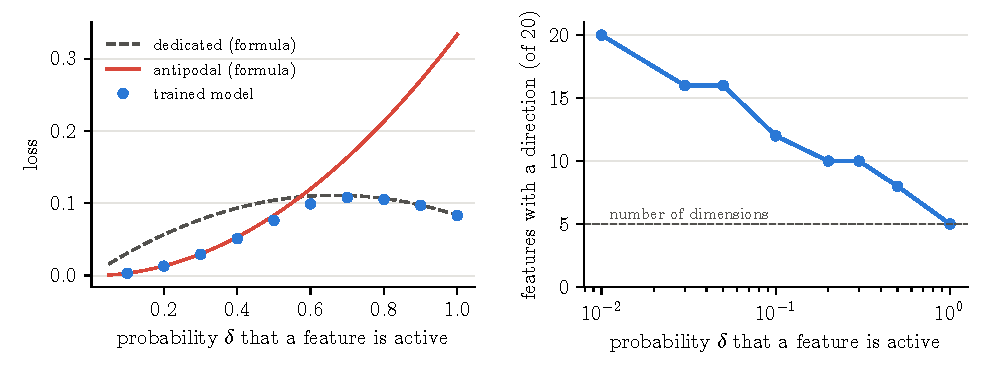
\includegraphics[width=0.95\textwidth]{figures/fig_toy_capacity.pdf}
\caption{Left: loss of the trained toy model with two features in one dimension, compared with the two formulas
of \cref{prop:toy} (\cref{exp:toytwo}). Right: number of features, out of 20, to which a trained model with 5
dimensions assigns a direction of norm above $0.5$.}
\label{fig:toycapacity}
\end{figure}

\subsection{Consequences}

If networks store features in superposition, three conclusions follow. They lead directly to the method of the
next
session.
\begin{itemize}
\item \textbf{Polysemantic neurons are expected.} If there are many more features than neurons, the feature
directions cannot all be aligned with the neurons. Then each neuron has a nonzero component along many feature
directions, and it responds to all of the corresponding features, as in \cref{exp:neurons}.
\item \textbf{We have to find the right units of analysis ourselves.} The features are directions, and no part
of the architecture tells us which directions they are.
\item \textbf{Finding the features is a sparse recovery problem.} We observe many activation vectors, and we look
for a set of directions, more numerous than the dimension, such that each activation vector is a combination of
only a few of these directions.
\end{itemize}

\begin{caution}
Superposition in small models like the one above is established. Superposition in large language models is
still a hypothesis. It is supported by indirect evidence: polysemantic neurons, the success of the sparse
autoencoders of session 5, and studies with probes that may use only a few neurons \citep{gurnee2023finding}.
Nobody has yet listed and counted the features of a real language model.
\end{caution}

\begin{takeaways}
Single neurons usually respond to several unrelated things. A high-dimensional space contains exponentially
many almost orthogonal directions, so a network can store far more features than it has dimensions. The cost is
interference, which stays small as long as only a few features are active at the same time. A small model trained
by gradient descent behaves exactly like this: it represents as many features as it has dimensions when the
features are dense, and many more features when they are sparse.
\end{takeaways}

\subsection*{Questions for the seminar}

\begin{exercise}[Three features in the plane]\label{ex:triangle}
Three features are stored in $d=2$ dimensions along unit vectors at mutual angles of $120^\circ$. Show that
$v_i^\top v_j=-1/2$ for $i\ne j$. Show that the read-out $\hat f_j=\relu(v_j^\top x)$ recovers $f$ exactly whenever
at most one feature is active. Which panel of \cref{fig:toygeometry} uses the same trick?
\end{exercise}

\begin{exercise}[Negative interference is scarce]\label{ex:negative}
(a) Let $v_1,\dots,v_N$ be unit vectors with $v_i^\top v_j\le-\varepsilon$ for all $i\ne j$, where
$\varepsilon>0$. Show that $N\le1+1/\varepsilon$. Hint: the squared norm of $v_1+\dots+v_N$ is not negative.
(b) Compare the result with \cref{prop:jl}. (c) The read-out of \cref{ex:triangle} removes negative interference
at no cost. Why can this trick alone not support a large number of features?
\end{exercise}

\begin{exercise}[Typical interference]\label{ex:typical}
(a) Let $v_1,v_2$ be independent random vectors, uniformly distributed on the unit sphere of $\R^d$. Show that
$\E\,(v_1^\top v_2)^2=1/d$, and compare with \cref{exp:random}. (b) Let $x$ be the sum of $k$ such vectors, and
let $v$ be one more. Show that $v^\top x$ has mean zero and variance $k/d$. (c) For $d=768$ and $k=40$, compare
$\sqrt{k/d}$ with the bound $k\varepsilon$ of \cref{lem:interference} for $\varepsilon=0.3$. What do we learn
about the lemma?
\end{exercise}

\begin{exercise}[Polysemantic without superposition]\label{ex:polysem}
Give an example of a layer with $d=2$ neurons and $N=2$ features that are represented in orthogonal directions,
in which both neurons are polysemantic. What does the example show about the relation between polysemantic
neurons and superposition?
\end{exercise}

\begin{readinglist}
\item \citet{gurnee2023finding}, \emph{TMLR}. Evidence for superposition in real language models, obtained with
probes that may use only a few neurons.
\item \citet{liu2025superposition}, \emph{NeurIPS}. Trains the toy model of this session with a controlled degree
of superposition and relates it to the way in which the loss of a model falls with its width.
\item \citet{arora2018linear}, \emph{TACL}. An early precursor: word vectors as sparse combinations of a large set
of directions for meanings.
\item The main source of this session, \citet{elhage2022toy}, is not peer reviewed. It is long, and its first
three sections are the best next reading after this session.
\end{readinglist}
